\chapter{Data processing}
STORM data from different cells or structures show many different features: there can be clusters of flourophores with a high density of spots, areas with low density, variable background in space and time, beads can be present or not. This section is about how the algorithm processes the data sets and how it is possible to find good settings that will work for all kind of input data.\newline
All real world images shown in this thesis were aquired from members of Prof. Dr. Mike Heilemanns group.


\section{Import and processing}
STORM data has usually a size of around 3 gigabytes. There are even larger datasets possible, so that it is important to work on smaller parts of the data, instead putting the whole dataset into memory. This is done using chunks of a user defined size. The data is processed chunkwise, and there is parallelisation for the frames of each chunk. This parallelisation is possible because the signals in each frame are considered to be independent from each other.  

\section{Workflow}
\subsection{Choosing parameters}
Initially the user has the option to set all important parameters. If no parameter is set the default ones are used and will give a good result because all crucial parameters are either determined from the data or set to reasonable values that work for every data set. The goal of the default parameters is to give a good result with no adjustment. This means parameters are chosen to produce almost 100 \% precision. The loss of some points that are not detected using this conservative setting will not affect the final result as much as a lower precision would.
\subsection{Estimating camera gain and offset}
First the application checks for a file containing settings for gain and offset from an earlier run. If this is not the case new parameters are estimated based on the first part of the data; usually 200 frames are sufficiant.\newline
The method described by \cite{skellam} is used to estimate the
gain factor. For this method a Skellam distribution is used. 
Each dataset is three-dimensional, where time is the third
dimension. Therefore mean $\mu$ and variance $\sigma^2$, in time, can be calculated from
the data for each pixel individually
\begin{align}
	\mu(i,j) & = \frac{\Sigma_t(I_t(i,j)-I_{t+1}(i,j))}{n}\\
	\sigma^2 & = \frac{\Sigma_t(\mu(i,j)-(I_t(i,j)-I_{t+1}(i,j)))^2}{n-1}
\end{align} 
$I_t(i,j)$ describes the intensity of the pixel of frame $t$ at position $i,j$.
To determine the gain factor the Skellam parameter are plotted over the mean
intensities. A straight line can be fitted, and its slope gives the gain
factor, the intersection is the offset.\newline 
The methode for the fit uses R \cite{Rcite}. To suppress outliers, the fit is performed only on a compact subset of all points \cite{ilia1}, more details can be found in the manual of SimpleSTORM \cite{ilia2}. This part of the algorithmn was developed and implemented by Ilia Kats.  
\subsection{Recursively adjusting gain and offset}
After the estimation of gain factor and offset, the transformations described in \ref{trafoPoiss} and \ref{trafoAnscombe} are applied and the background is subtracted.\newline
Due to the Anscombe transformation, the background pixels of the image should only vary around a mean intensity of zero with a variance of 1. Therefore, a histogram of the pixel intensities is created. After background subtraction, the background pixels should contribute only to the lower intensities in the histogram. A gaussian function is fitted to the histogram's values. This is done under the assumptions that there is much more background in the image than signal, or that the intensities coming from signals are distributed over a larger range, so the Gaussian for the background intensity distribution can be fitted correctly.\newline
If the estimated value for the variance is too far from 1, the originally estimated gain factor is corrected and applied, and the fit is done again. This is done until the background variance converges or the maximal number of iterations is reached. In this case the initial gain factor will be used and a warning printed to the screen.
\subsection{Estimating the width of the point spread function}
For a certain number of frames, the Fourier transform is calculated and averaged. The result is called the mean power spectrum. It can be used to estimate the variance of the point spread function of the signal. A two dimensional Gaussian function's Fourier transform is again a Gaussian but with inverse variance. This relation is used to determine the variance of the point spread function in the spatial domain, using the fit parameter for the variance in the frequency domain.\newline
The script for fitting the two dimensional Gaussian function was implemented by Ilia Kats.
\subsection{Processing the data}
\subsubsection{Import Data}
Storm data sets can consist of several thousand frames with resolutions up to one mega pixel per frame. This size makes it necessary to break the data into smaller parts because otherwise it might be much larger than the RAM of an ordinary machine. Because of the background estimation, it is not possible to process every frame completly independently as it was in the older version of this software (\cite{MAJoachim}). It is also faster with some datatypes to load a larger consecutive part of the dataset into memory.\newline
This algorithm uses chunks of user defined size. There are some limitations to the chunk size that are discussed later. The data set is split into parts of equal size in the $x$- and $y$-dimensions and independently also in the $t$-dimension. If this partition does not fit at the edge of the data set, the last chunks will be smaller.\newline
The data is transformed to be Poission distributed, then the Anscombe transform is applied. After the Anscombe transformation the background intensities have unit variance.\newline
The implementation of the workflow using chunks was implemented by Ilia Kats.
\subsubsection{Background estimation}
For each chunk, the median of the Anscombe transformated data is determined to get a robust estimate of the background value for this chunk. 
B-spline interpolation, implemented in vigra (\cite{vigra}), is used to get interpolated values for the full resolution of the current frames. For this interpolation, three chunks in both the spatial and the temporal domain have to be available. Therefore the maximal chunk size into $t$-dimension must not be larger than a third of the total stack size, the same holds for the chunk size in $x$ and $y$ direction which must not exceed the spatial resolution of the image stack.\newline
This background is then subtracted from the transformed data to give finally background pixels with zero mean and unit variance, both in $xy$- and in $t$-dimension. Figure \ref{removedBG} shows an frame with variable background before and after background subtraction.
\begin{figure}
\subfloat[Original image]{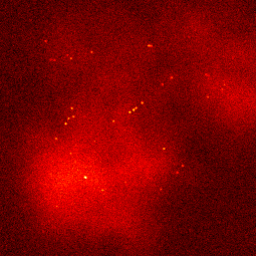
\includegraphics[width = 0.485\textwidth]{pictures/Tubulin2OrigFrame50Color.png}}\hfill
\subfloat[image after background subtraction]{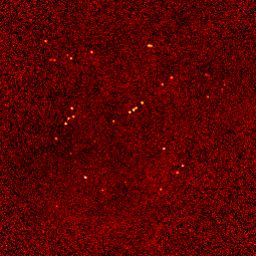
\includegraphics[width = 0.485\textwidth]{pictures/Tubulin2normalprocessFrame50Color.png}}
	\caption{Effect of background subtraction on inhomogenous background. For the human eye no more points are visible but for computers it is much easier to find the bright spots in the background subtracted image, because a global threshold can be applied.}
	\label{removedBG}	
\end{figure}
\subsubsection{Create mask for background suppression}
With the given $p$-value from the settings, a global threshold can be determined, because inhomogenities of background intensities have been removed. The threshold value is that intensity that is explained from a Gaussian distribution with mean zero and variance one with the given $p$ probability. This is possible because the background intensity follows such a distribution after all the applied transformations.\newline
The threshold is applied to the current frame and stored as a mask. Due to the probability that background pixels intensitis might exceed the threshold the connected components of the mask are calculated. Pixels that belong to connected components with too few members are discarded. The idea behind using connected components is, that there is a probability for a background pixel to be brighter than the threshold, but it is unlikely that two neighbouring pixels exceed the threshold in the same frame and even more unlikely that three of them does. Therefore the number of pixels necessary for not discarding a connected component is set to three at least. If the width of the point spread function is very large the number of pixels can be set depending on the psf width. But to suppress background pixels efficiently it has to be larger than three.
\subsubsection{Filtering data and finding maxima}
To improve the accuracy of the spot detection, the transformed signal is convolved with a two dimensional Gaussian function with the previously determined or user-set width. The convolved image will further be used to find the maxima. Each maxima found is tested to be covered by the mask or discarded otherwise. A region of interest around the remaining maxima is interpolated to a higher resolution. The interpolated region is searched for maxima for the last time. This maxima will be detected with super resolution.\\
To determine the signal-to-noise ratio, the unfilterd and uninterpolated pixel intensity is used.

\subsubsection{Quality control for detections}
Sometimes, especially in data sets with a high density of spots, two spots are near enough that their point spread functions overlap. It may happen that instead of two maxima just one maximum will be detected right between the true ones, as it can be seen in \ref{betterthansimplestorm}. This leads to large errors in the localisation. To avoid this a threshold for the asymmetry of the spots can be set.\newline
The calculation of the asymmetry was already implemented by Joachim Schleicher \cite{MAJoachim}.


\section{Comparison with older version of the SimpleStorm algorithm}
\subsection{Adjustable filter width} \label{sectionFilterisEvil}
If two or more point spread functions (PSF) overlap, applying a smoothing filter can lead to merging point spread functions. This merging becomes a problem if the two distinct maxima of the original unsmoothed PSFs form a new maxima in between, which leads to just one detection somewhere between the true maxima. The number of merging psfs increases with greater filter widths. For high density data, it might be better to use a filter with smaller width and therefore with less accuracy, but with fewer merged PSFs. In total this might give a better result depending on the number of incorrectly merged PSFs. This is the reason why the filtering was changed to use just a Gaussian filter instead of the Wiener filter originally used. 
The effect of the smaller filter width can be seen in Figure \ref{betterthansimplestorm}. The red crosses indicate detections found by the new SimpleStorm version, the green crosses show the estimated positions from the previous version of SimpleStorm, and the white x marks the ground truth. The predictions by the newer version are not perfect but better than the predictions of the older version. The scores of the two prediction can be seen in Table \ref{tabelbetterthansimplestorm}. Both results have almost the same accuracy, but they differ in the scores. There are two effects canceling each other out related to the accuracy. Fewer merged PSFs increase the accuracy, but the positive effect of filtering with the appropriate filter, as shown in \ref{accplot2} or in \ref{matchedFilter1}, is also lost. 

\begin{table}
\caption{Comparison of results created using almost no smoothing or Wiener filter on high density data. Although the accuracy is almost the same, the number of detections and the scores are higher for the unsmoothed data. For the evaluation, software from the \cite{challenge} were used.}
\begin{tabular}{l|llllll}
&intersections&Jaccard&F-Score&Precision&Recall&RMSE\\ \hline
Gaussian filter, width = 0.01& 16955&19.99&33.26&81.10&20.92&27.21\\
Wiener filter& 14480&17.06&29.15&79.19&17.87&27.28
\end{tabular} \label{tabelbetterthansimplestorm}

\end{table}


\begin{figure}
\subfloat[Advanced setting widget]{
\includegraphics[width = 0.485\textwidth]{pictures/betterthanSimplestorm1.png}}\hfill
\subfloat[Easy setting widget]{
\includegraphics[width = 0.485\textwidth]{pictures/betterthanSimplestorm2.png}}
	\caption{This pictures show the effect of a smaller filter width. The red crosses show detections found with a filter width of 0.01, the green crosses the results using a Wiener filter. The white x marks the ground truth.}
	\label{betterthansimplestorm}	
\end{figure}

\subsection{False positive suppression}
In the previous version the background was determined by first estimating a baseline, the minimum of the current frame was taken. This baseline was subtracted and the resulting image smoothed with a gaussian filter of widht 10. The smoothed image was subtracted from the original image to give a background free image. This works fine for subtracting background with variations larger than the filters width, but gives as a result just intensities without any information about the variability of the background intensities. If for example the resulting intensity, after background subtraction is 5, this can either mean it is definitly signal if the variance of the background in the original image was very small, but it can also mean nothing, if the variance of the original background was 20, the probability that the difference of 5 between the original image and the smoothed one has a high chance to result from the background variation.\newline
In the older version of SimpleSTORM the intensity of a candidate, that was considered to be signal, was checked by comparing its intensity after the background subtraction with its intensity before. If the maximums intensity was at least twice as high as the subtracted background it was taken for further processing, otherwise discarded. If the background has a high variability in the spatial domain, the baseline gets a value that is too low for the regions with a higher mean intensity. For this regions the background that is subtracted has high values and therefore the maxima are discarded because the resulting intensity is lower than the twice the background. This phenomena can be seen in figure \ref{bgmakesitbad}. The old version of SimpleSTORM just findes about 8000 spots while the new version finds more than 44000. This results in a better reconstructed image that shows the underlying structure in a better way.

\begin{figure}
\subfloat[Typical frame showing variable background intensities]{
\includegraphics[width = 0.3\textwidth]{pictures/Tubulin2OrigFrame50.png}}\hfill
\subfloat[Result old SimpleSTORM]{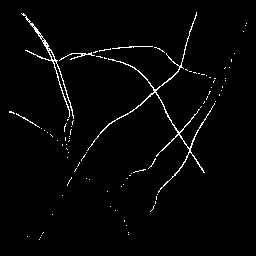
\includegraphics[width = 0.30\textwidth]{pictures/Tubulin2factor1OldSimpleSTORM.png}}\hfill	
\subfloat[Result new SimpleSTORM]{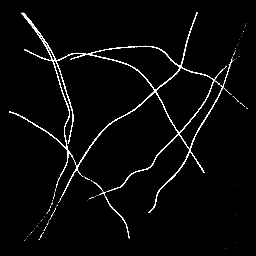
\includegraphics[width = 0.3\textwidth]{pictures/Tubulin2factor1.png}}

\caption{This pictures show the drawback of the old background treatment. On the left a typical frame with variable background is shown. The old version of SimpleSTORM discards many detections in the regions of high background intensity. The new SimpleSTORM software discards detections based on their signal-to-noise ratio and is less affected by variable background.}
\label{bgmakesitbad}	

\end{figure}

The great advantage of the newer version of SimpleStorm is its model for the background. For each pixel, the probability to be signal can be determined based on its signal to noise ratio (SNR). Using the number of connected components of each cluster, false positive detections caused by bright background pixels can be suppressed. This is a great advantage over background suppression methods that work just on intensities.

\subsection{Comparable results based on the signal-to-noise ratio}
The accuracy of the maxima detection relies on the signal to noise ratio. With a given SNR the correct standard deviation of the localisation error can be used for further calculations. This is not possible if just an intensity is saved because without information about the backgrounds variance the reliability of the detection can't be estimated.\newline
To save the signal-to-noise ratio is also an advantage when results are compared that result from either different cameras or different settings or a different environment that might lead to a higher background variability. 


\section{New graphical user interface (GUI)}
\subsection{Input widget}
The new GUI for SimpleStorm was designed because of its many new features. Figure \ref{guiWidgets} shows the new design. The GUI was mainly designed by Ilia Kats.
There are three categories of parameters. The first category specifies which upsampling factor shall be used or what is the pixel width of the input data, is given in nanometers. This is information that can be given by any user without knowing anything about the algorithms  the SimpleStorm software uses. The most challenging parameter of this section is the alpha value, which sets the sensitivity for false detections. If the user doesn't know what this means or which values gives the best results, they can use the default setting and alternate it after the run. \newline
The next category of parameters is about region of interest (roi) widths for the estimation of the point spread function and chunk sizes. There are two different ways to set these parameters (see Figure \ref{guiSettings}). One way is to give values for all parameters. This is difficult without understanding the influence of these parameters on the algorithm. Therefore there is also a second way to set this parameters. The user should know some properties of the data that shall be processed, such as: is the spot density high or low? Is there variable background in time and space? Depending on the sliders' positions, the best parameters are set automatically. How this is done will be described later. With this second option the user can process his or her data, treating variable background or dense data without deep insight or understanding of the algorithms.\newline
The last catagory of parameters describes the camera gain and offset, the width of the signals point spread function, and a prefactor that can be used to alter the estimated gain. 
\begin{figure}
\subfloat[Easy setting widget]{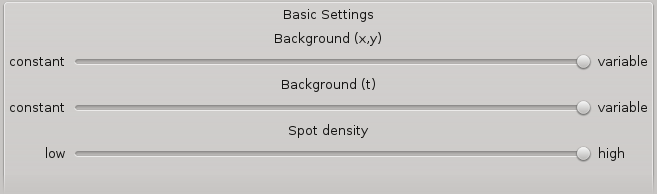
\includegraphics[width = 0.485\textwidth]{pictures/basicSettingsGui1.png}}
\subfloat[Advanced setting widget]{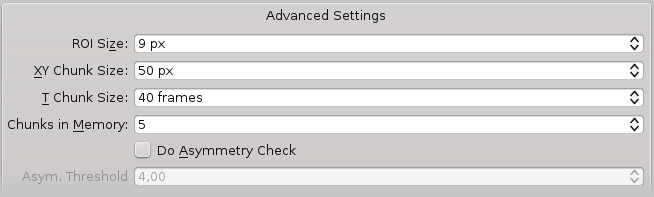
\includegraphics[width = 0.485\textwidth]{pictures/advancedSettingsGui.png}}\hfill
	\caption{There are two different ways to set the parameters important for the algorithm. On the right the standard way of setting parameters can be seen. On the left, there are sliders that can be adjusted between two extremes. The program sets the value for the parameters in a way to produce the best results for the selected attributes of the data set.}
	\label{guiSettings}	
\end{figure}
\subsection{Result widget}
After the run button at the lower left edge of the input widget is pressed, a new tab opens. In this widget the reconstructed image is shown. At the bottom there is a progress bar that displays the current processing step and its progress. Buttons to zoom in and out or to fit the displayed image best into the window are located in the lower part of the result widget. On the lower right there is the stop/save button. It either stops the program if it is still runing or opens a dialog to save the result image and the coordinates of the detection if the program has already been stopped.

\begin{figure}
\subfloat[Input widget]{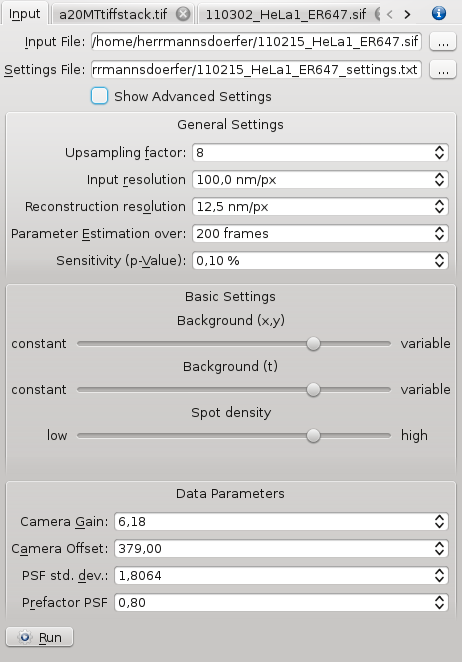
\includegraphics[width = 0.405\textwidth]{pictures/InputWidget.png}}\hfill
\subfloat[Result widget]{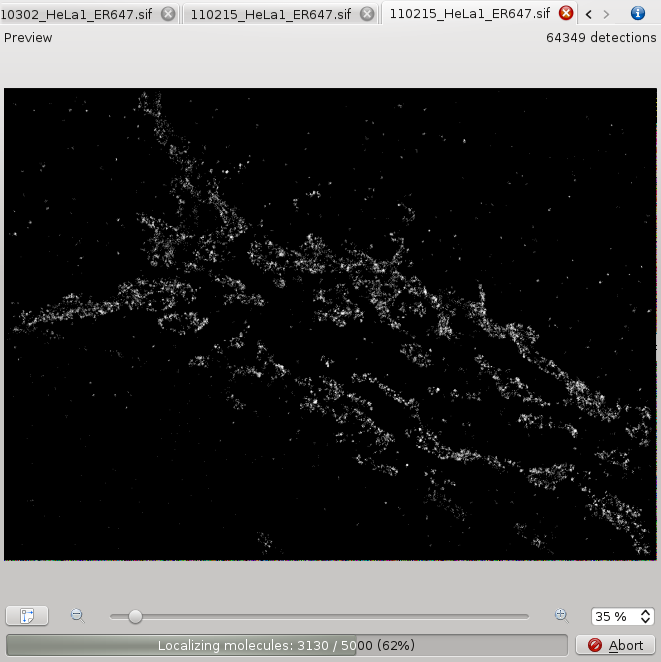
\includegraphics[width = 0.575\textwidth]{pictures/ResultWidget.png}}
	\caption{The new GUI. On the left is the window for selecting input file and parameters. On the right is the result widget showing the processing of a data set in progress.}
	\label{guiWidgets}	
\end{figure}

\subsection{Easy parameter selection}
As mentioned above, with the easy setting widget it is easy to set reasonable parameters without knowing their influence on the algorithms.\newline
The background sliders have direct influence of the corresponding chunk size. A more constant background gives better results with larger chunks. This is the case because the median of all pixels in a chunk is used to estimate the mean value of the background. For this estimation this relation between the median and the mean $\lambda$ of a Poisson distribution is used
\begin{align}
\text{median Pois} \approx \lambda +\frac{1}{3} - \frac{0.02}{\lambda}
\end{align}
Because of the high mean values for $\lambda$ the last summand is dropped.
Therefore the chunks have to contain more background pixels than signal, otherwise the mean value will be overestimated. With large chunks this assumption is satisfied. But the smaller the chunk size the more likely it is that a cluster of points lies in the chunk, and because of that the median gives too high values. On the other hand, the chunk sizes should be in the range of the changes in background. The best chunksize is therefore in the range of the variable background. The slider position sets the chunk sizes linearly to a value that lies in between the smallest chunk size possible and the largest chunk size possible for the data set. The minimal possible chunk sizes are 3 pixels, and the largest chunk size possible is the the half of the shorter border in $x$ and $y$ dimension and the number of of frames over which the parameters are estimated divided by the number of chunks in memory in $t$ dimension.\newline 
In general, the more dense the dataset is, the more likely it is that two neighbouring PSFs are merged due to the filtering, as showed in \ref{sectionFilterisEvil}. There are two ways to avoid inaccurate detections. One is less filtering, to avoid merges, the second one is checking the symmetry of the detected spots. Merged spots become more and more asymmetric the further the two true centers of the PSFs lay apart from each other. A high asymmetry is a good indicator for a poorly detected spot.
The spot density influences the prefactor for the estimated sigma and the value for the asymmetry checks. It sets the threshold for the asymmetry in the same way the sliders for background work, within appropriate limits, with higher values for less dense data sets. Also, the prefactor is set to values between 1 for sparse data and zero for dense data.